
%%%%%%%%%%%%%%%%%%%%%%% file typeinst.tex %%%%%%%%%%%%%%%%%%%%%%%%%
%
% This is the LaTeX source for the TDPTemplate using
% the LaTeX document class 'llncs.cls' Springer LNAI format
% used in the RoboCup Symposium submissions.
% http://www.springer.com/computer/lncs?SGWID=0-164-6-793341-0
%
% It may be used as a template for your own TDP - copy it
% to a new file with a new name and use it as the basis
% for your Team Description Paper
%
% NB: the document class 'llncs' has its own and detailed documentation, see
% ftp://ftp.springer.de/data/pubftp/pub/tex/latex/llncs/latex2e/llncsdoc.pdf
%
%%%%%%%%%%%%%%%%%%%%%%%%%%%%%%%%%%%%%%%%%%%%%%%%%%%%%%%%%%%%%%%%%%%

\documentclass[runningheads,a4paper]{llncs}
\usepackage{amssymb}

\setcounter{tocdepth}{3}
\usepackage{graphicx}
\usepackage{amssymb}
\usepackage[utf8]{inputenc}
\usepackage{url}
\usepackage{float}
\usepackage{amsmath}
\usepackage{graphicx}
\usepackage{wrapfig}
\usepackage{tabto}
\usepackage{lipsum}
\usepackage[table,xcdraw]{xcolor}
\usepackage{hyperref}
\usepackage[french]{babel}
\begin{document}
\selectlanguage{french} 


\newif\ifdraft
\draftfalse


\ifdraft
\setlength{\belowcaptionskip}{-5pt}
\fi

\title{Walking Machine @Home \newline \: Rapport de projet 2018}

\author{Jeffrey Cousineau and Philippe La Madeleine}
\institute{École de Technologie Supérieure \\ 1100 rue Notre-Dame Ouest, Montreal, QC, Canada H3C 1K3 \\
\texttt{http://walkingmachine.ca,} \texttt{walking@ens.etsmtl.ca,} \texttt{https://github.com/WalkingMachine}}
\maketitle


%%%%%%%%%%%%%%%%%%%%%%%%%%%%%%%%%%%%%%%%%%%%%%%%%%%%%%%%%%%%%%%%%%%%%%%%%%%%%%%%%%%%

\begin{abstract}
Ce papier donne des détails à propos du projet de l'équipe Walking Machine de l'école de technologie supérieure, participant à la compétition Robocup@Home.  Leur prochaine compétition se déroulera à Montréal, dans leur ville natale. Le robot du club Walking Machine se nomme S.A.R.A. pour "Système d'assistance robotique autonome". Ce robot est entièrement conçu par le regroupement de passionnés et est principalement composé d'élève du 1er cycle en génie. Leur robot est utilisé pour l'interaction humaine et l'assistance personnelle. Ce document démontrera les différentes avancées technologiques apportées dans la dernière année au niveau logiciel, électrique et mécanique.

\end{abstract}

%%%%%%%%%%%%%%%%%%%%%%%%%%%%%%%%%%%%%%%%%%%%%%%%%%%%%%%%%%%%%%%%%%%%%%%%%%%%%%%%%%%%

\section{Introduction}

L'équipe de Walking Machine est une jeune équipe de Montréal et composée de jeunes étudiants dans le domaine du génie mécanique, électrique et logiciel. Elle a beaucoup travaillé au niveau de l'amélioration du robot pour la prochaine année afin de participer pour une troisième fois à la compétition Robocup@Home. Après quelques années d'expériences, il y a eu un très grand apprentissage, ce qui en résulte en de de belles améliorations qui mèneront à de meilleurs résultats, principalement du côté logiciel. Dans le passé, l'équipe a participé à plusieurs compétitions comme la Eurobot mais, a décidé de changer afin de faire face à un plus grand défi et ainsi, d'avoir l'opportunité d'apporter une vague d'innovation dans le monde scientifique entourant la robotique. \\

S.A.R.A. fut conçue pour une interaction humain-robot polyvalente et une navigation efficace. La plateforme robotique est équipée de roue mecanum et de moteurs maxon alimentés par des drives Roboteq. Elle a également un bras permettant d'immiter un bras humain ainsi que des capteurs pour la communication et la navigation. Notre équipe a développé une certaine expérience dans la reconnaissance de visages et d'objets en plus de la navigation utilisant un laser 2D. Ces différents modules sont interfacés via ROS (Robot Operating System). \\

\section{Améliorations électriques et mécaniques}
\subsection{Électrique}

Comme amélioration cette année du côté électrique de notre robot, nous avons mis beaucoup d'efforts sur l'organisation de l'élaboration du système en le rendant plus clair et sécuritaire. Nous avons donc ajouté des protections pour chaque sous-système électrique puisqu'il est ainsi beaucoup plus facile de changer un fusible qu'un circuit complet. \\

Un autre gros changement pour nous fut le système de batterie. Tout juste avant de partir pour notre compétition au Japon en juillet 2017, nous avons changé notre ancienne batterie LiPo maison par des batteries de perceuse. Ce changement a apporté beaucoup plus de points positifs que prévus. Tout d'abord, cela a simplifié l'exportation internationale de notre robot et nous permettait d'emmener les batteries dans nos bagages personnels. Le deuxième impact majeur fut le sentiment de sécurité qui accompagnait ce type de batterie. Il est beaucoup facile de les charger et sécuritaire puisque ce type de batterie possède possède leur propre chargeur adapté avec des circuits de protection. De plus, notre système à deux batteries instauré dans  notre robot nous donne la possibilité d'enlever une des deux batteries sans avoir à éteindre le système complet.\\



\subsection{Mécanique}

Quelques améliorations mécaniques furent également complétées durant l'année. Il y a principalement deux aspects qui furent repensés, soit le bras ainsi que la base.\\

Tout d'abord, l'année passée, notre bras possédait cinq degrés de liberté, ce qui rendait la planification de trajectoire beaucoup plus complexe et limitait grandement les mouvements. Nous avons donc décidé de rajouter deux degrés de liberté grâce à deux servo-moteur Dynamixel. Depuis cette modification, nous avons des résultats grandement améliorés et une plus grande liberté de mouvement. Cela a également comme impact de rallonger le bras ce qui nous donne un plus grand rayon d'action.\\

\begin{wrapfigure}[10]{r}{0.20\textwidth}
	\centering
	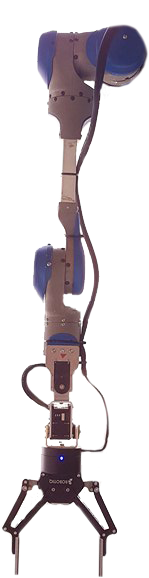
\includegraphics[width=0.10\textwidth]{images/arm.png}
	\caption{Bras à 7 degrés de liberté}
\end{wrapfigure}

L'autre aspect principal qui fut amélioré était la base de notre robot. Suite à notre première compétition en Allemagne, nous avons observé que la base était beaucoup trop large, ce qui causait quelques problèmes au niveau de la navigation autonome près des portes. En se basant sur ces observations, nous décidé de réduire la largeur ce qui a eu pour effet d'améliorer grandement les capacités en navigation. \\
\newpage
\section{Logiciel}

\subsection{Planification des tâches de haut-niveau}
Pour notre planification des tâches que notre plateforme pouvait accomplir, nous avons utilisé un module développé par une équipe de robotique participant à la compétition Darpa Robotics Challenge. Ce logiciel nommé \href{http://philserver.bplaced.net/fbe/index.php}{FlexBe}\cite{schillinger2016flexbe}, pour Flexible Bahavior, est composé d'une interface de style programmation par blocs, il est donc facile et clair d'implémenter les différents scénarios pour la compétition.\\


\begin{figure}[h!]
	\centering
	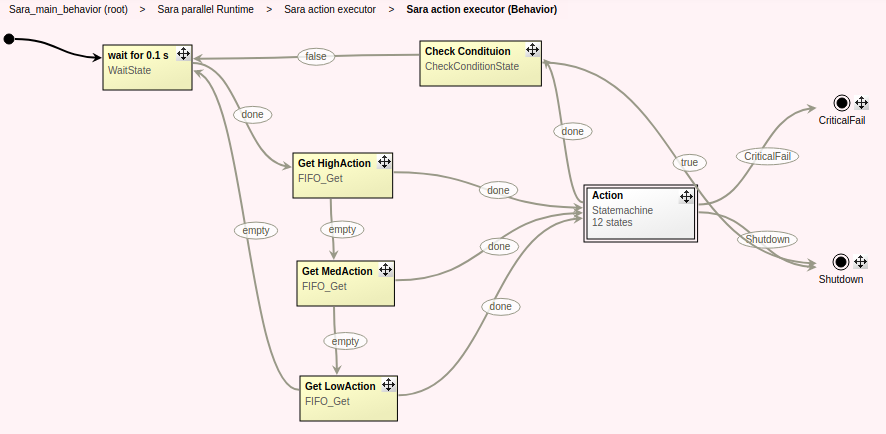
\includegraphics[width=0.70\textwidth]{images/flexbe.png}
	\caption{Représentation de FlexBe}
\end{figure}

Par contre, nous n'utilisons pas tout simplement FlexBe, nous devons programmer nos propres états en utilisant l'API en python. Pour simplifier notre travail, nous avons commencé par diviser tous les scénarios de base demandé lors de la compétition Robocup@Home en petites actions reproductibles. Nous avons ensuite repérées ceux pouvant être accomplies par notre robot et les avons transformée en état (ex : mouvement du bras à une position X). Ces blocs d'état peuvent ensuite être assemblés ensemble pour former une hierachie plus élevée que l'on nomme Actions. Nous assemblons finalement ces actions en ActionWrapper qui permettront d'interfacer les actions générale de notre robot avec la détection vocale ainsi que le traitement du language. Ces différents modules interpêtent ainsi le language et le transforme en action réalisable par le robot. Cette structure récursive nous permet donc un développement beaucoup plus rapide pour chaque tâches nécessaires. \\

\subsection{Natural language processing}
\tab To analyze the detected speech, we rely on a software develop by the  \href{http://sag.art.uniroma2.it/}{Semantic analytic group from the University of Roma} and the \href{http://labrococo.dis.uniroma1.it/}{Laboratory of Cognitive Cooperating Robots} at Sapienza University of Rome. This speech analyzer, named \href{http://sag.art.uniroma2.it/lu4r.html}{LU4R}\cite{lu4r} for “Language Understanding For Robots”, is composed of a server developed in Java which takes as an input the detected sentence and the semantic environment surrounding the robot.\\

This server communicates through a REST service which gives it the possibility to be compliant with all kind of platform. All you have to do is to launch the server locally which is compiled through a .jar file. Again, this gives the opportunity to use this software on every platform, whether you’re on Windows, Linux or Mac. This software gives you the possibility to get different output representation. We choose the \href{https://github.com/amrisi/amr-guidelines/blob/master/amr.md}{amr representation} since it was the easiest one to understand and to implement.\\

We decided to build our own ROS wrapper, \href{https://github.com/WalkingMachine/lu4r_ros}{lu4r\_ros}  to better interface it with our task planning approach. We first translate the answer given by LU4R into the simple format, we call ActionForms. The ActionForms contains an action followed by all of its possible parameters as identified in the \href{https://framenet2.icsi.berkeley.edu/fnReports/data/luIndex.xml}{FrameNet Index of Lexical Units}
The ActionWrappers are then fed into a FIFO based priority manager and finally send to our task planner.\\

What is also interesting about LU4R, it’s that it will use the semantic mapping in it’s analyzing process. All you have to do is to provide the correct pose for every object in the robot’s environment. You can also precise various synonym for every object to get a better understanding of the inputted sentence.\\


\subsection{Object recognition}
\tab As a beginning team, we are still exploring various solution around the object recognition problem. Our first plan was to use the object recognition kitchen package from Willow Garage. But after using it in competition, we realized that the performance and the easiness to use wasn’t the approach we were looking for. As an alternative, we start using the YOLO\cite{yolo} (You Only Look Once) ros package. \\

YOLO is a real-time object detection. It does not only detect various object but it also predicts the bounding boxes of the detected object. It uses a single neural network which is applied to the image. Multiple regions are then created and are used to predict the bounding boxes. Each of them also contains the predicted probability which is used to filter the predicted objects. The advantage of this system is that it can detect multiple objects in a real-time scenario.\\
 
\begin{figure}
  \centering
  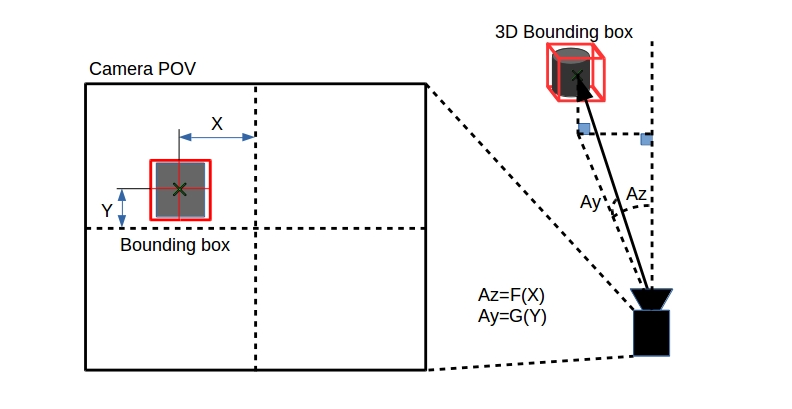
\includegraphics[width=200pt]{images/frame_to_box.png}
  \caption{2D bounding box to 3D grasping pose, current technique}
\end{figure} 
 
We use the ROS package to make our job easier since this gave us the possibility to directly get the recognized objects output into a ROS topic. We can also get the bounding box for each detected object. First step we had to do was to transform those 2D bounding boxes in 3D to get a specific pose according to our robot. \\

For the moment, we created the package \href{https://github.com/WalkingMachine/wm_frame_to_box}{wm\_frame\_to\_box} to approximate the object pose with the depth point at the center of the bounding box. Even though it can have flaws, this technique has also proven to be largely sufficient for most of our applications and most importantly, it uses way less processing power than the full 3D pattern matching we used before. This allows us to do real-time object positioning, a capability we are proud of.\\

Afterward, to get better results and a better pose, we plan to subtract the point cloud according to the bounding boxes. We will then use it with the pointcloud segmentation from the \href{http://pointclouds.org}{PCL library} to extract the specific object and send it to a grasp identification package like \href{http://http://wiki.ros.org/haf_grasping}{haf\_grasping}. This technique, compared to what we are actually using would give us the possibility to grab a much wider variety of object.\\

\begin{figure}
  \centering
  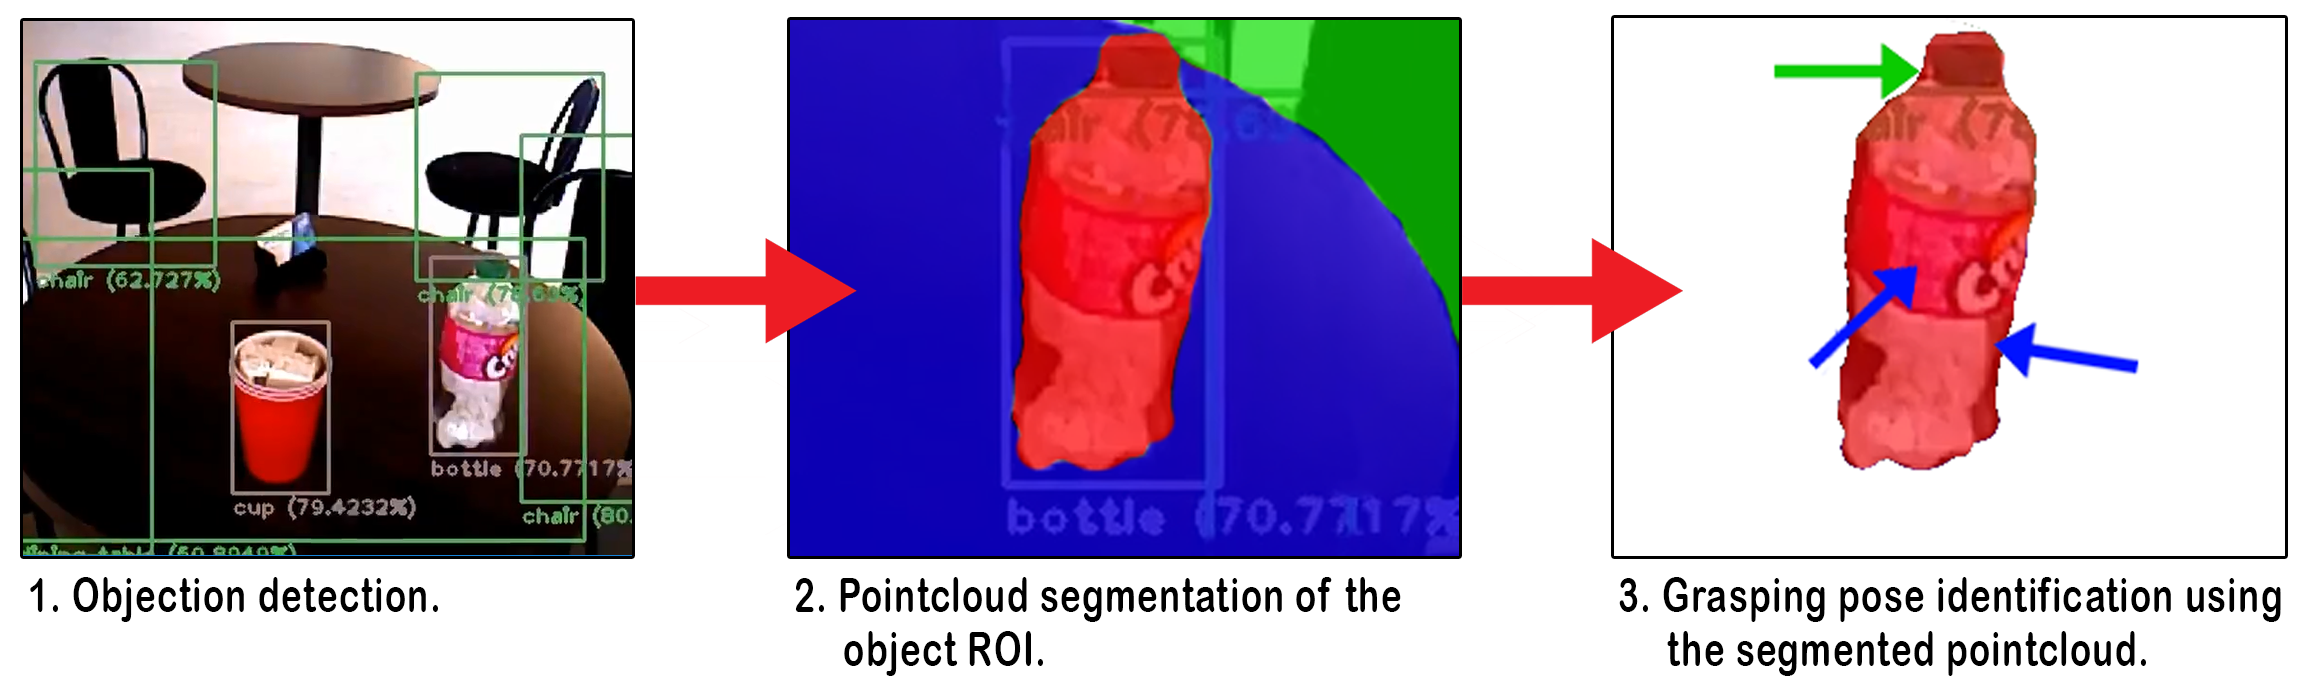
\includegraphics[width=300pt]{images/frame_to_box2.png}
  \caption{2D bounding box to 3D grasping pose, future technique}
\end{figure}

For the moment, we are using the YOLO model but, we are looking forward to training our own dataset, just like we would do in competition. This is new for us but we have all the tools we need to overcome this. \\

\subsection{Navigation}
En plus de notre système de navigation précédemment utilisé, cette année nous utilisons le module \href{http://wiki.ros.org/pointcloud_to_laserscan}{pointcloud\_to\_lasercan} comme solution plus légère afin de faire de l'évitement d'objets en 3D. Cela nous assure une navigation beaucoup plus sécuritaire puisqu'en utilisant seulement une navigation 2D à l'aide d'un lidar, il serait possible que le robot entre en collision avec une table puisqu'il ne verrait que les pattes de celle-ci. Un autre avantage de cette implementation est qu'il est possible de spécifier la hauteur maximum au niveau des collisions. Ainsi, nous évitons également les possibles collisions avec la tête de notre robot. \\

\subsection{Représentation de l'environnement}
Comme nouveauté cette année, nous avons implémenté notre propre solution afin de représenter l'environnement entourant le robot d'une façon simple pour tout le monde. Notre solution que nous avons nommée \href{http://github.com/walkingmachine/wonderland}{wonderland} est un système agnostique dans le même genre que LU4R présenté plus tôt. Il est composé d'un serveur recevant une requête HTTP basée sur un API développé par l'équipe.\\

La première choses requise pour commencer à utiliser cette plateforme, est l'action de populer la base de donnée. Cela peut être fait de façon manuelle en indiquant la position de chaque objet connu, mais cela peut être fait par le robot à l'aide de requête POST. Il est également possible de spécifier une pièce avec une position relative à celle-ci. Lorsque les différentes informations sont insérées, il est possible de faire une requête GET sur l'adresse définissant le serveur de wonderland (ex : http://wonderland:8000/object). Cette dernière retournera la liste complète des objets contenue dans la base de donnée. Il est également possible de filtrer les demandes en rajoutant par exemple une couleur ou une position comme paramètre. \\

Puisque la base de donnée est hébergée sur un serveur, il est possible d'y accéder de puis n'importe où. Il est possible de l'exporter sur un autre ordinateur, de la mettre en infonuagique ou seulement de l'installer sur l'ordinateur même du robot. Cela donne également la possibilité d'avoir une connaissance dynamique, ce qui signifie que le robot peut mettre à jour ses connaissances de l'environnement en temps réel.\\



\section{Conclusions et projets futures} 
Comme vous pouvez le constater, malgré que nous soyons une équipes composée principalement d'étudiants de premier cycle, nous sommes tout de même capable de rivaliser avec les autres équipes composées de laboratoire de recherche. Nous avons recemment mis beaucoup d'effort afin d'avoir une plateforme plus stable et de réduire les différents bogues présents, nous permettant donc d'avancer dans la bonne direction. \\

Avec notre nouveau système de batteries interchangeables, notre détection d'objets et l'inteprétation du language naturel, notre robot devient est devenu une plateforme autonome complètement fontionnelle, nous permettant donc de nous concentrer sur le coeur des challenges de la compétition.\\

\section*{Robot SARA Hardware Description}
% TODO Change picture and description
Specifications for robot SARA are as follows:

\begin{table}

\label{my-label}

\begin{tabular}{l|p{90mm}}
\hline
\rowcolor[HTML]{FFFFFF} 
\multicolumn{2}{c}{\cellcolor[HTML]{FFFFFF}\textbf{SARA}}                                                      \\ \hline
\rowcolor[HTML]{EAEFF6} 
\textbf{Base}               & Custom base with fully holonomic platform                                        \\
\rowcolor[HTML]{FFFFFF} 
\textbf{Right arm}          & 7 DoF custom arm made of Kinova motors                                           \\
\rowcolor[HTML]{EAEFF6} 
\textbf{Neck}               & Tilt and pan unit using two Dynamixel MX-64R servo actuator                      \\
\rowcolor[HTML]{FFFFFF} 
\textbf{Head}               & Custom head made of RGB neopixels leds and Asus Xtion Pro                        \\
\rowcolor[HTML]{EAEFF6} 
\textbf{Gripper}            & Robotiq 2 fingers 140mm                                                           \\
\rowcolor[HTML]{FFFFFF}
\textbf{Dimensions}         & \begin{tabular}[c]{@{}l@{}}Base : 0,61m. X 0,77m.\\ Height : 1,68m.\end{tabular} \\
\rowcolor[HTML]{EAEFF6} 
\textbf{Weight}             & $\sim$60kg                                                                      \\
\rowcolor[HTML]{FFFFFF} 
\textbf{Additional sensors} & Hokuyo UTM-30LX on base                                                          \\
\rowcolor[HTML]{EAEFF6} 
\textbf{Microphone}         & Rode microphone											                         \\
\rowcolor[HTML]{FFFFFF} 
\textbf{Batteries}          & 2x 20V Dewalt drill battery 5aH                                                 \\
\rowcolor[HTML]{EAEFF6} 
\textbf{Computer}           & 1x Lenovo p50 with 32GB RAM and nVidia Quadro M2000 4GB, 1x Raspberry Pi 3       \\ \hline
\end{tabular}
\caption{Robot's hardware description}
\end{table}
\begin{wrapfigure}[10]{r}{0.25\textwidth}
	\centering
	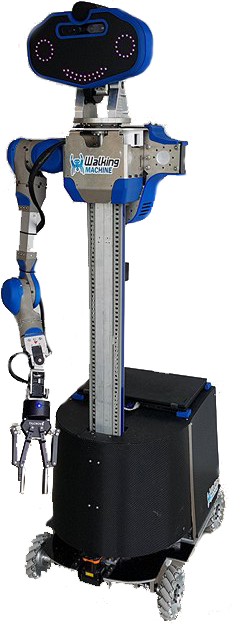
\includegraphics[width=0.30\textwidth]{images/sara_2.png}
	\caption{Robot SARA}
\end{wrapfigure}
\section*{Robot's Software Description}

For our robot we are using the following software:

\begin{itemize}
	\item Platform: Robotic Operating System (ROS) Kinetic on Ubuntu 16.04
	\item Navigation, localization and mapping: \href{http://wiki.ros.org/gmapping}{Gmapping}, \href{http://wiki.ros.org/amcl}{AMCL}, \href{http://wiki.ros.org/pointcloud_to_laserscan}{pointcloud\_to\_laserscan}
	\item Face recognition: \href{http://wiki.ros.org/people}{People}
	\item Speech recognition: \href{https://github.com/WalkingMachine/lab_ros_speech_to_text}{Google Speech API}
	\item Speech comprehension: \href{http://sag.art.uniroma2.it/lu4r.html}{LU4R}, \href{https://github.com/WalkingMachine/lu4r_ros}{lu4r\_ros}
	\item Speech generation: \href{https://doc.ubuntu-fr.org/svoxpico}{Svoxpico}
	\item Object recognition: \href{https://github.com/WalkingMachine/wm_darknet}{Darknet with YOLO v2 }
	\item Arm control: \href{http://wiki.ros.org/moveit}{MoveIt} and \href{https://github.com/Kinovarobotics/kinova-ros}{Kinova API}
	\item Task executor: \href{http://wiki.ros.org/flexbe}{Flexbe} 
	\item World reprensentation: \href{http://github.com/walkingmachine/wonderland}{Wonderland}
\end{itemize}
	

\section*{Membres de l'équipe}
Jeffrey Cousineau, Philippe La Madeleine, Maxime St-Pierre, Nathalie Connolly, Jimmy Poirier, Léonore Jean-François, Samuel Otis, Redouane Laref, Louis-Charle Labarre, Lucas Maurice, Nicolas Nadeau, Simon Landry, Cheuk Fai Shum, Veronica Romero Rosales, Nicolas Bernatchez, Quentin Gaillot, Raphael Duchaine, Jean-Frederic Boivin 

\nocite{*}
\bibliographystyle{plain}
\bibliography{references}


\end{document} 
